%!TEX root = ../thesis.tex
%*******************************************************************************
%****************************** Evaluation Chapter *********************************
%*******************************************************************************

\chapter{Evaluation}
\label{chap:evaluation}
In the previous chapter, we explained the implementation of our tool. 
Based on that, in this chapter, we will discuss the details of the evaluation process, including a user study we performed. 
Firstly, we explain the experimental design (see section \ref{evaluation:section:design}), which focuses on the planning and design of the user study. 
Next, we explain the execution section (see section \ref{evaluation:section:execution}) that involves the actual implementation of the study. 
Next, we explain the analysis section (see section \ref{evaluation:section:analysis}) discussing the processing of the data collected during the study and the results of the study. 
Finally, in the interpretation section (see section \ref{evaluation:section:interpretation}), we aim to draw conclusions from the analysis and determine the study's implications.
For the setup, we recruited participants from \ac{upb}\footnote{Website of Paderborn University: \url{https://www.uni-paderborn.de/}}.
\ifpdf
    \graphicspath{{Chapters/Evaluation/Figs/}{Chapters/Evaluation/Figs/}{Chapters/Evaluation/Figs/}}
\else
    \graphicspath{{Chapters/Evaluation/Figs/}{Chapters/Evaluation/Figs/}}
\fi

\section{Experimental Design}
\label{evaluation:section:design}
The experimental design is a crucial aspect of any user study as it determines the effectiveness and reliability of the study.
In conducting and reporting our user study research, we followed the established guidelines of Runeson and Höst \cite{eval:guidlines:runeson} (see figure \ref{evaluation:fig:casestudy}) to increase the quality of the study outcomes.
The experimental design comprises three main components: defining an objective, user scenario and research questions, establishing a study protocol, and addressing ethical concerns.

% To evaluate the effectiveness of our approach, we conducted a case study that involved recruiting participants, developing prototypes, and working on user scenarios. 
% We recruited 15 participants who are students at Paderborn University. 
% The case study is based on the evaluation stage of the first cycle of our DSR (as discussed in section \ref{introduction:section:research}).
% These guidelines helped ensure our research was rigorous, transparent, and credible. 
% By adhering to these guidelines, we aimed to provide a detailed and comprehensive account of our case study, enabling others to replicate our research and build upon our findings.
% This case study also aims to develop the RQ as explained in the next section.
% In this section, as per Runeson and Höst, we first define the objective, case study, research questions, and the methods we follow to complete the evaluation.

\paragraph{Objective:}
The user study aims to evaluate the usability and effectiveness of our model-based UI prototyping experimentation approach. 
Additionally, the study aims to identify any usability issues or limitations of the approach through user testing. 
Furthermore, the study aims to test the effectiveness of the \ac{dp}s suggested by our approach in terms of the participants' ease of use and understandability. 
Through the evaluation, we hope to gain insights into the strengths and weaknesses of the approach and provide recommendations for further improvement.
Based on these objectives, we define some \ac{rq}s in the next section.

\begin{figure}[ht]
  \centering
  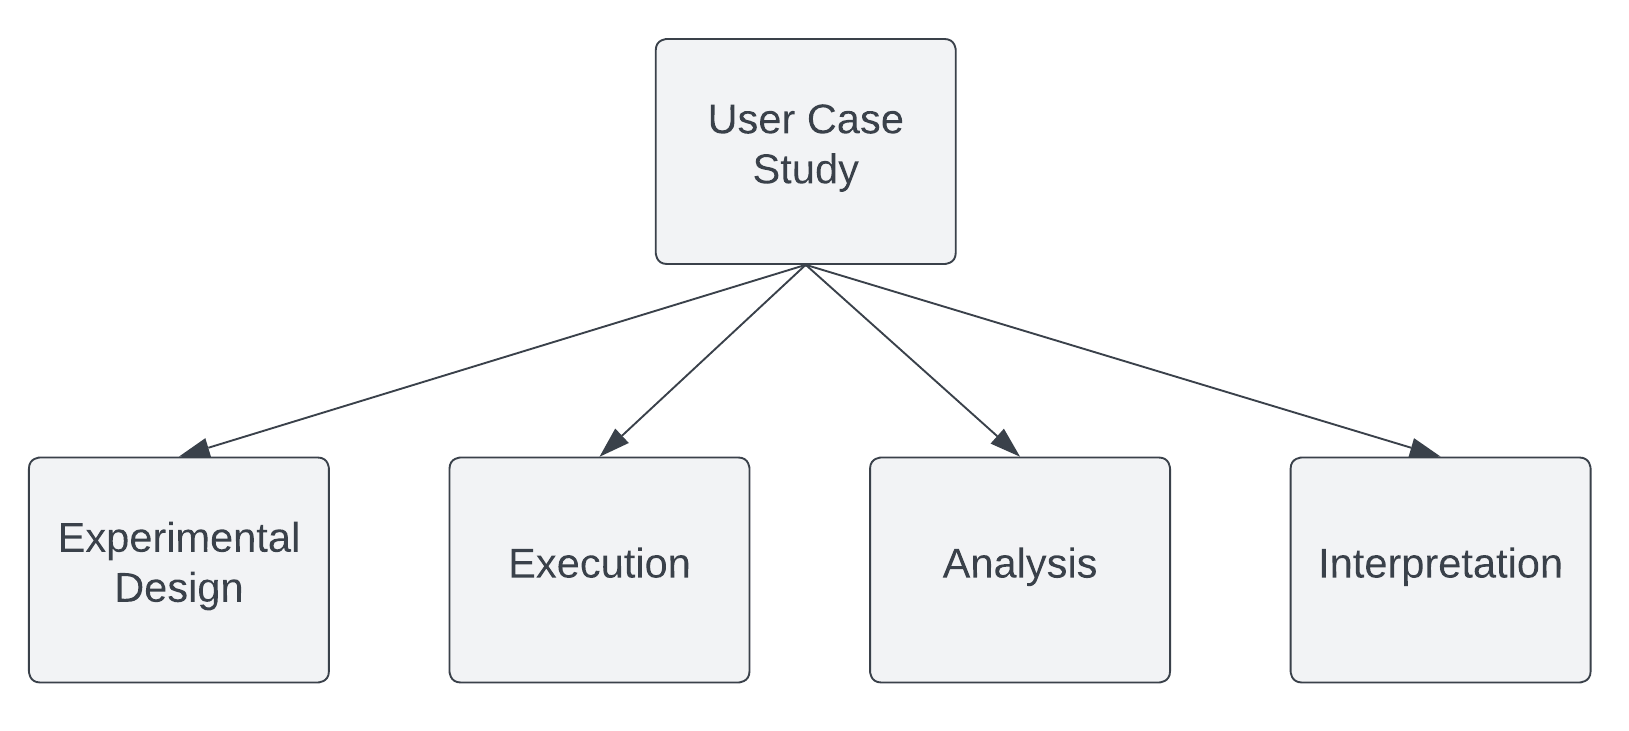
\includegraphics[scale=0.25]{case-study.png}
  \caption{User Case Study for Analysis}
  \label{evaluation:fig:casestudy}
\end{figure}

\paragraph{Research Questions:}
Based on the main \textit{\hyperref[introduction:section:research]{\ac{rq}}}, we defined a couple of research questions for the user study. \\
\textbf{RQ1:} How effective is the model-based UI prototyping experimentation approach in enabling product designers to conduct experiments on UI prototypes independently of developers? \\
\textbf{RQ2:} What \ac{dp}s are suitable for product designers to develop UI prototypes in the model-based UI prototyping experimentation approach?

\paragraph{Study Protocol:}
For the user study, we aimed to recruit diverse participants from different courses enrolled at \ac{upb} to ensure a wide range of perspectives and experiences on UI prototyping and UI Experimentation. 
We wanted to include individuals with varying experience in prototyping and user scenario development, from beginners to experts.
To recruit participants, we first sent an invitation message and email (see figure \ref{evaluation:fig:invitation}) to our research group and other groups at the university. 
The invitation message included a Doodle\footnote{Website for Doodle: \url{https://doodle.com/}} link, an online tool for setting up the appointment.
The potential study participants clicked on the link and selected a one-hour slot for the study. 
After booking the slot, the participants received a detailed invitation email  (see appendix \ref{appendix:three:caseStudy} for details), which specified the location of the study, prerequisites, and a user scenario.
\begin{figure}[ht]
  \centering
  \begin{tcolorbox}[title=\texttt{From: Rakshit\\ To: various groups\\ Subject: Invitation to Participate in a User Study}]
  Hello,\\
    
  my name is Rakshit Bhat, and I am inviting you to participate in my user study, which is a part of my master's thesis evaluation. 
  The study is based on a UI prototyping tool with an option to create different UI variants and find the best fit for the prototype.
  Your participation in this study will greatly help me evaluate the effectiveness and contribute to advancing UI prototyping tools.\\

  The study will require about \textit{45-60} minutes, during which you will be asked to perform some tasks using the tool and provide your feedback.\\
  Your participation in this study will be highly appreciated.\\
  If you are interested in participating, please schedule a session using the Doodle link at your convenience. (Please try to select the empty spots)\\
  If these slots do not fit you, you can always contact me, and we can find some slots.\\

  After selecting the slots, an invitation email will be sent to you with further details.\\
  Thank you for considering.\\
  
  \textbf{Link for Doodle:}
  <<Doodle Link>>
    
  Cheers,\\
  Rakshit
  \end{tcolorbox}  
  \caption{Recruiting the Participants for User Study}
  \label{evaluation:fig:invitation}
\end{figure}

Since our tool was hosted online at the \ac{upb} server, we used \ac{bbb}\footnote{Website for BBB: \url{https://open-bbb.uni-paderborn.de/}}, an open-source web conferencing system, to monitor participants during our user study.
We chose \ac{bbb} because it is easy to use, reliable, and provides all the required features for our study. 
We conducted the study remotely, and \ac{bbb} allowed us to interact seamlessly with the participants during the study. 
As the \ac{bbb} service is also provided by our \ac{upb}, we did not have to worry about additional costs or compatibility issues. 
Therefore, \ac{bbb} was a valuable tool for monitoring the participants during our study.

For our user study, there were a few prerequisites that the participants needed to fulfill. 
Firstly, since our tool was hosted on the \ac{upb} server, participants were required to have access to the \ac{vpn}\footnote{Website for University Paderborn VPN config: \url{https://imt.uni-paderborn.de/vpn-zugang/}} to access the tool. 
The \ac{vpn} ensured that only authorized individuals could access the tool.
Secondly, the participants needed a good internet connection as the tool was web-based and required a stable internet connection for smooth functioning. 
Lastly, although the participants did not need any prior experience with \ac{ui} prototyping or \ac{ui} experiments, they required very basic knowledge, which we also explained before starting the study. 
It ensured they could understand the tasks and provide meaningful feedback during the study.

After finishing the user scenario, the participants were asked to fill out a questionnaire to provide us the qualitative and quantitative feedback.
This questionnaire was created using Limesurvey\footnote{Website for UPB hosted Limesurvey: \url{https://umfragen.uni-paderborn.de}}, an open-source online survey tool that is a service provided by UPB for surveys. 
The questionnaire consisted of three parts. 
The first part included the \ac{sus}, a standardized questionnaire for assessing the usability of a system. 
The second part included a Likert scale (1-5) for participants to rate the effectiveness of our \ac{dp}s in improving the usability of the prototyping experimentation approach. 
In the third part, we included three open-ended questions to gather qualitative feedback from participants on the strengths, weaknesses, and suggestions for improvement of the approach.

% We developed a user scenario that required participants to use our UI prototyping tool hosted on the Paderborn University server. 
% Therefore to access our tool, the participants needed to turn on the VPN\footnote{Website for University Paderborn VPN config: \url{https://imt.uni-paderborn.de/vpn-zugang/}} provided by the University. 
% We also examined them using an open BigBlueButton\footnote{Website for BBB: \url{https://open-bbb.uni-paderborn.de/}} video conference session. 
% We also considered the ethical clarifications by informing the participants that we were not recording the video conference session and that the survey was anonymous to ensure their privacy and encourage honest feedback while mentioning our data collection and storage strategy.

% After using the tool, participants were asked to answer a questionnaire in the survey to provide qualitative and quantitative feedback for our tool and the \ac{dp}s we developed. 
% The questionnaire was designed to evaluate the usability, effectiveness, and overall satisfaction with our tool. 
% We also asked for suggestions for improvement and gathered additional comments and feedback from the participants to gain a deeper understanding of their experiences.


\paragraph{User Scenario:}
To conduct the user scenario, we gave the participants a hypothetical situation where they had to imagine themselves as John, a UX designer, creating a movie-streaming app. 
We then guided them through a set of tasks to prototype the UI and create split or A/B tests to select the best variant. 
Finally, we asked them to gather feedback through a set of questionnaires and monitor the results to see which version of the app's interface was more effective.

\paragraph{Ethical considerations:}
Finally, for ethical considerations, we took steps to ensure the privacy and anonymity of the participants. 
During the user study, we used BBB and informed the users that we were not recording the session. 
We only stored the user's department at the university to ensure diversity in the user case study. Additionally, we made the survey questionnaire anonymous to ensure participants could answer honestly without fear of repercussions. These steps confirmed that the user study was conducted ethically and respected the participants' privacy.

\clearpage
\section{Execution}
\label{evaluation:section:execution}
The execution phase of our user study involved several key steps. 
We conducted pilot testing to ensure our user scenario was well-designed and effective. 
Following this, we recruited participants through various channels and scheduled one-hour appointments with each of them. 
During these appointments, we collected data and observed as the participants executed the user scenario we had created. 
In this section, we will discuss each of these steps in more detail, including our pilot testing, recruitment, and data collection process. 
We will also provide an example scenario to illustrate one participant's experience with our prototyping tool.

\paragraph{Pilot Testing:}
Before the actual execution of the user study, we conducted pilot testing to ensure that the user scenario and the tool were easy to understand and use. 
Initially, we did the pilot testing ourselves to identify potential issues and gather feedback. 
Later, we also asked two friends to test the tool and scenario to get additional feedback.
Based on the feedback during the pilot testing, we made some updates and improvements to the tool and the user scenario. 
We addressed the bugs pointed out to us and made some changes to improve the tool's usability. 
The changes were made to ensure the participants' smooth experience during the actual user study.

\paragraph{Recruitment:}
Recruitment is an essential part of conducting a user study as it determines the quality and representativeness of the data collected. 
After completing the pilot study, we initiated the recruitment process for our user study. 
We sent an invitation email to various groups and channels that we believed would be interested in participating. 
The email included a Doodle link where potential participants could select their preferred time slots.
The study lasted one hour for each participant, and as the participants selected different slots, the entire user study continued for two weeks. 
After agreeing to participate and giving their verbal consent, we sent the user scenario to each participant.
We received a response from 17 participants who agreed to participate and selected their preferred slots for the study. 
Unfortunately, two participants later backed out for reasons beyond our control. 
After reading the user scenario, one participant did not like the study, and another fell sick before their scheduled slot.
The recruitment process was conducted carefully to ensure that we had a diverse range of participants. 
We confirmed that the participants represented different departments in the university to ensure we had a good mix of perspectives. 
We also ensured that the study was voluntary and participants could opt out at any point. 
We provided anonymity for all participants by not recording any personal information, and we also ensured that the survey questionnaire was anonymous.


\paragraph{Data Collection: User Participation and Observation}
For the data collection step, firstly we started the \ac{bbb} session at the appointed time, and the participant joined us. 
Before beginning the session, we informed the participant that we would not be recording the session. 
We then asked the participant to share their screen while executing the user scenario.
During the session, we observed the participant performing the scenario and took notes wherever necessary. 
We made sure to inform the participant before the start of the session that we would be taking notes to avoid any discomfort. 
The first two participants had doubts about the scenario, so after their participation, we had to update the scenario to improve it. 
The remaining thirteen participants had slightly different scenarios from the first two.
After completing the scenario, we asked the participant to stop sharing the screen and answer the questionnaire or the survey on Limesurvey. 
The survey questionnaire was anonymous to maintain the participants' confidentiality. 
The survey asked questions about the user's experience and the tool's usability.
After the session, we thanked all the participants for their valuable time and participation in our study. 
After the successful participation of all 15 candidates, we gathered all the notes and survey responses for analysis.

% \paragraph{Planning:}
% Before conducting the user case study, we carefully planned the experimental design to ensure the validity and reliability of our results.
% First, we defined a hypothesis to be tested. We wanted our POC tool to fulfill the Design principles and validate the DPs. 
% To achieve this, we developed a user scenario that involved the participants using our tool to create a prototype and conduct a user scenario. 
% We recruited diverse participants enrolled in various courses at Paderborn University, with varying experience in prototyping and user scenario development.
% To recruit participants for our case study, we shared a Doodle link via different communication channels, such as email and social media. 
% The Doodle link contained the necessary information about the study, including the purpose, duration, and requirements. 
% It also offered different time slots for the participants, ensuring that the survey could accommodate a diverse group of participants with varying schedules. 
% This method helped us efficiently reach out to potential participants and allowed them to select a time that suited them best.

% Secondly, we used the Lime survey, hosted on the Paderborn University server, to conduct a survey questionnaire to collect qualitative and quantitative feedback from the participants. 
% The questionnaire was divided into three sections. 
% The first section contained the \ac{sus} questionnaire, a widely used and reliable tool for measuring the usability of software systems. 
% This section aimed to collect quantitative feedback from the participants regarding the usability of our prototype tool. 
% The second section contained questions about the design principles we proposed in our thesis. 
% This section aimed to collect participants' ratings and opinions on the effectiveness and feasibility of the design principles. 
% The third section contained open-ended questions to gather participants' qualitative feedback and suggestions for improving our prototype tool and the \ac{dp}s. 
% We used the Lime survey to facilitate the data collection process and to ensure anonymity and privacy for the participants.

\paragraph{Example scenario:}
The scenario was that John, a UX designer, was creating a new movie-streaming app and wanted to prototype different UI designs and conduct split tests to select the best variant. 
The study was conducted in several phases.
In the first phase, John explored the tool and generated an example movie streaming prototype using the headstart button. He then added new movies to the prototype using the data model feature.
\begin{figure}[ht]
  \centering
  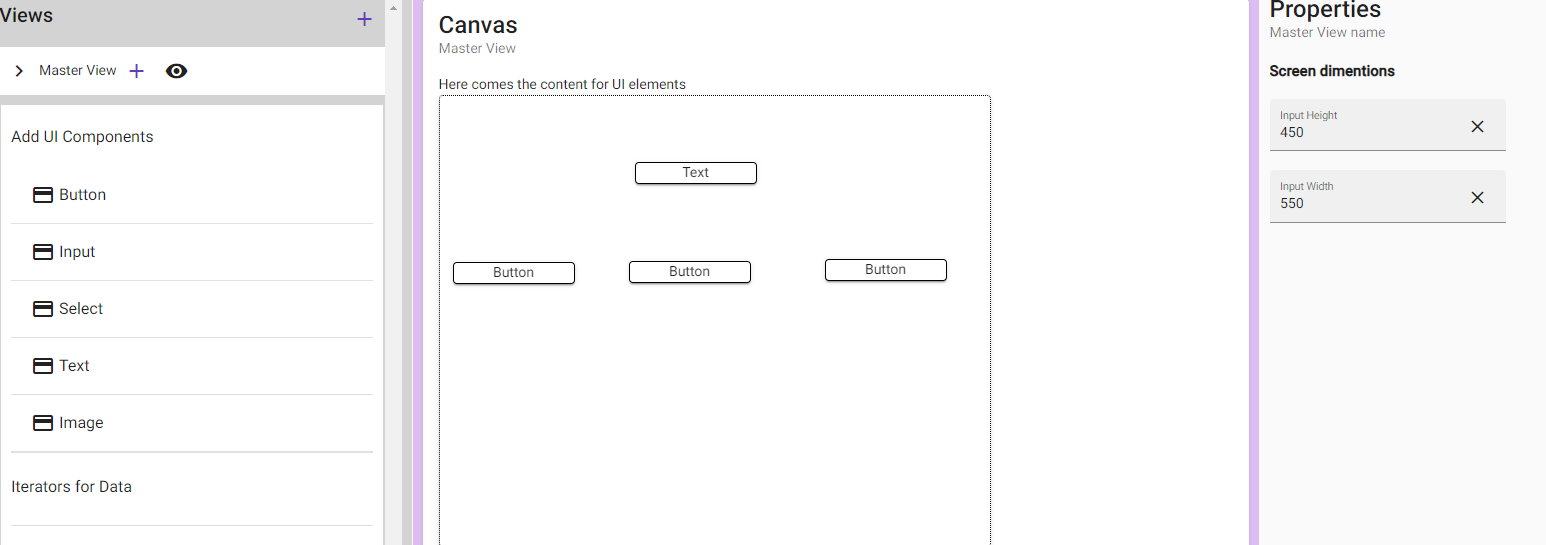
\includegraphics[scale=0.4]{MasterView.png}
  \caption[Example Participant Prototype - Screen1]{Participant Master View}
  \label{evaluation:fig:masterview}
\end{figure}

In the second phase, John created split tests for different app interface versions. 
He used the tool's A/B testing feature to create two versions of the app's view screen and changed the UI to make some changes in the variant's prototype.
\begin{figure}[ht]
  \centering
  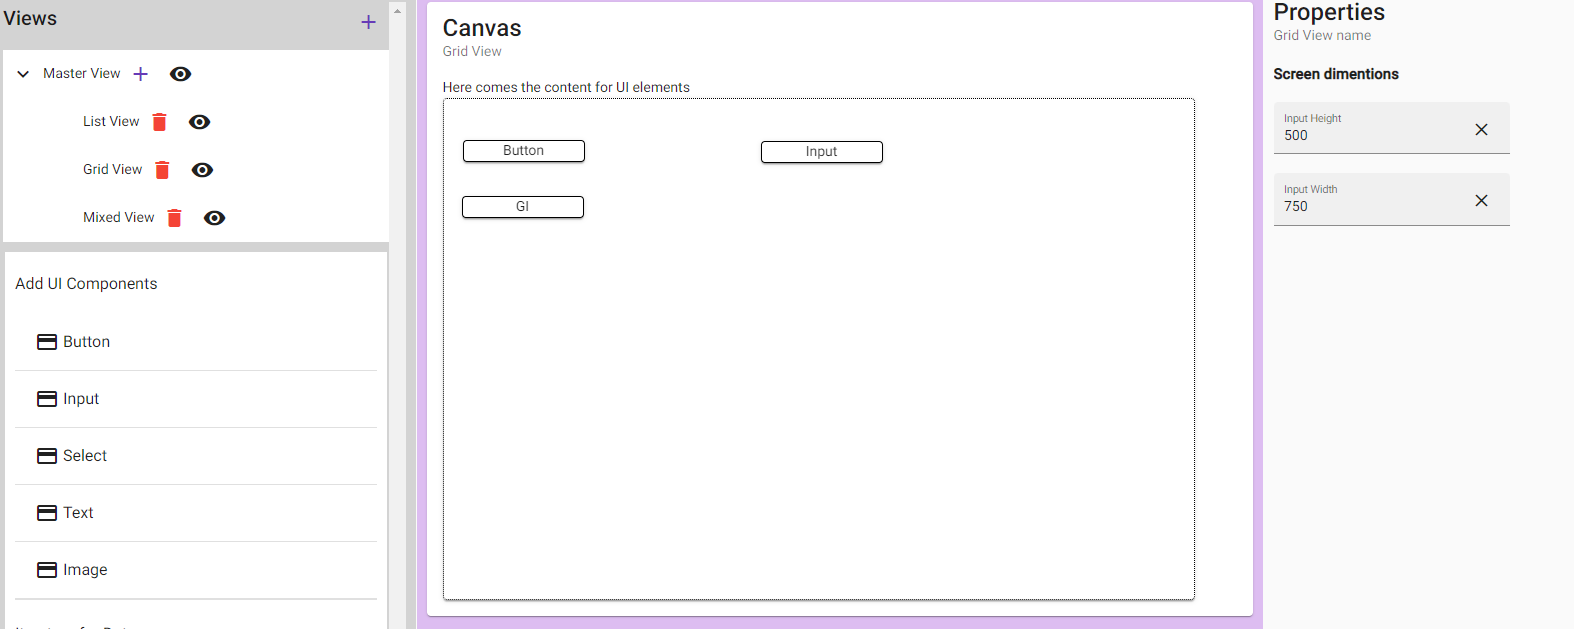
\includegraphics[scale=0.35]{GridView.png}
  \caption[Example Participant Prototype - Screen2]{Participant Grid View}
  \label{evaluation:fig:gridview}
\end{figure}

In the third phase, John created tasks for participants to complete and gather feedback on the app's interface. 
He also created a set of questionnaires, including open-ended and scale-based questions, to collect qualitative data from participants.
In the fourth phase, John recruited participants or used dummy users generated from the tool to test the experiments and monitor the results. 
After completing the experiment, John navigated to the experiments page and analyzed the statistics to determine which version of the app's interface was more effective.
Based on the feedback from the usability tests and questionnaires, John iterated on the app's design and updated the prototype in the tool. 
Overall, the execution of the experiment involved prototyping, split testing, task creation, and feedback gathering to design and improve the movie-streaming app's interface. 
An example prototype, created by one of the user participants, is shown in figures \ref{evaluation:fig:masterview}, \ref{evaluation:fig:gridview}, \ref{evaluation:fig:listview}.
\begin{figure}[ht]
  \centering
  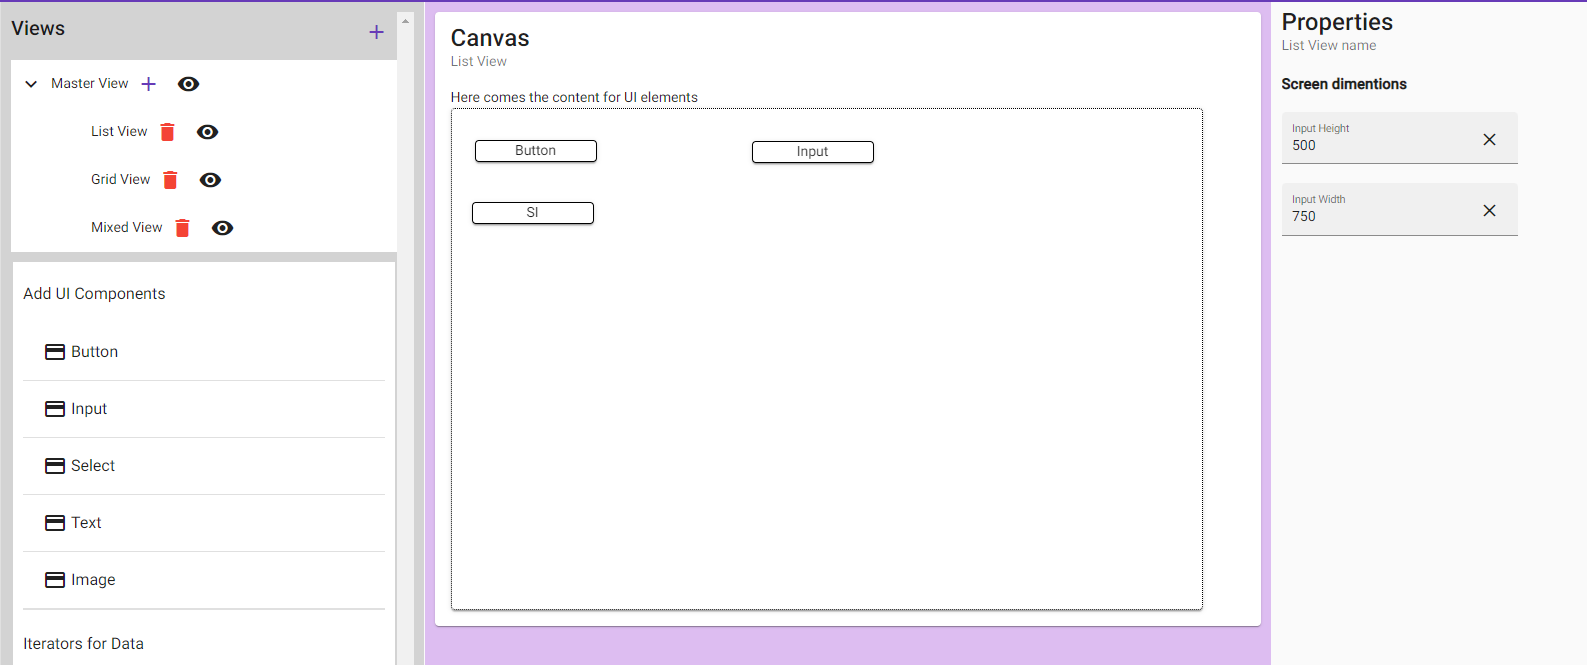
\includegraphics[scale=0.35]{ListView.png}
  \caption[Example Participant Prototype - Screen3]{Participant List View}
  \label{evaluation:fig:listview}
\end{figure}
\clearpage
\section{Analysis}
\label{evaluation:section:analysis}
After collecting the data through LimeSurvey and the tool, we analyzed the feedback and results to draw insights and conclusions about the effectiveness of our research questions and the software tool we designed.
The analysis phase of the user study is an essential part of the research process that helps to interpret the collected data and draw meaningful conclusions. 
This section includes the four steps in the analysis phase: data preparation, data reduction, quantitative analysis, and qualitative analysis.
We also examined the qualitative feedback from the participants to gain a deeper understanding of their preferences and needs. 
Next, we explain the qualitative and quantitative analysis of the data collected from the participants in detail.

\paragraph{Data Preparation:}
We focused on data preparation in the first step of the analysis phase. 
We collected data from different sources, including the notes taken during the BBB session and the survey responses collected using Limesurvey. 
We first organized and cleaned the data to make it ready for analysis. 
This step involved going through the notes and categorizing them based on the difficulties faced by participants, bugs observed during scenario execution, and ambiguity in the scenario. 
We also exported the survey responses from Limesurvey, which were in raw form and needed to be organized to accumulate the data for analysis.
We used the export feature of Limesurvey to get the survey responses from each participant. 
However, the data was per participant, and we needed to accumulate the data to analyze it. 
For example, the SUS values from section one must be collected for all participants to get an overall view of the system's usability. 
Therefore, we had to spend some time organizing the data and getting it in a format that would be easier to analyze. 
We used MS Excel to compile and accumulate the data. 
This process required attention to detail, as we needed to ensure we had all the necessary data in the correct format to draw meaningful conclusions. 
Once we had organized the data, we moved on to the next step of the analysis phase, which was data reduction.

\paragraph{Data Reduction:}
Data reduction is the next step in our user study's analysis phase. 
The data we collected needed to be reduced to the most important aspects for analysis. 
One of the key aspects was the \ac{sus} scores. 
The \ac{sus} score provided a numerical value indicating the tool's usability level. 
We also analyzed the responses to the open-ended questions in the survey to gain a deeper understanding of the participants' experiences. To group the responses from the open-ended questions, we categorized them into different themes. 
Additionally, we focused on analyzing our \ac{dp}s as they were the foundation of our tool's design. 
By prioritizing the most important data for analysis, we gained meaningful insights into our tool's usability and identified improvement areas.
Once we had reduced the data, we moved on to the next step of the analysis phase, which was data analysis including qualitative and quantitative.

\paragraph{Quantitative Analysis}
\begin{figure}[ht]
    \centering
    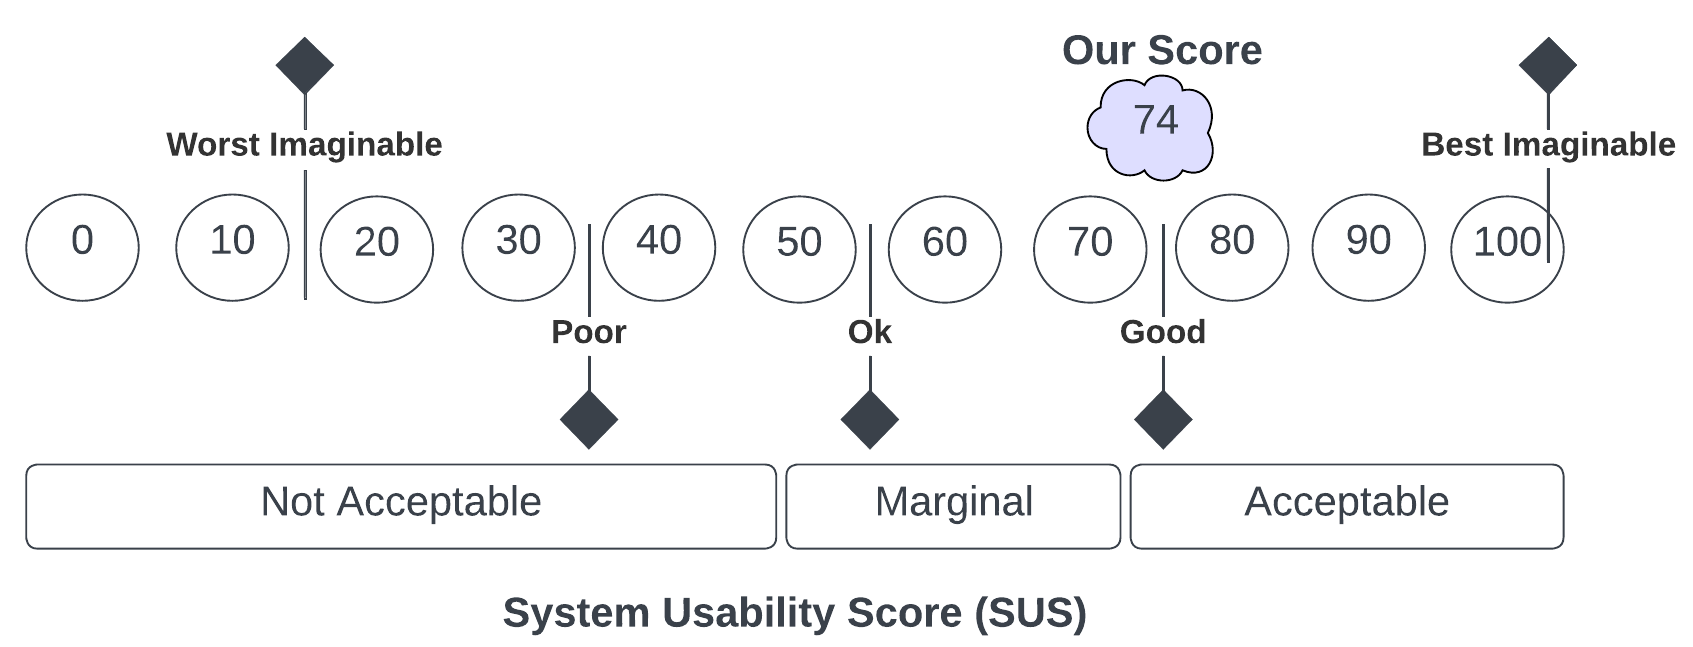
\includegraphics[scale=0.25]{SUS.png}
    \caption{System Usability Score of Our Tool}
    \label{evaluation:fig:sus}
\end{figure}
In the first part of the quantitative section of our analysis, we utilized the \ac{sus} to gather feedback on the usability of our tool. 
The \ac{sus} is a widely used and well-established questionnaire for assessing the usability of a system. 
It consists of 10 statements that participants rate on a 5-point scale from 1 (strongly disagree) to 5 (strongly agree). 
The scores from each report are then combined and transformed to create a final \ac{sus} score ranging from 0 to 100.
After administering the \ac{sus} questionnaire to our participants, we computed the average score to obtain a quantitative measure of the usability of our tool (for raw data see Appendix \ref{appendix:three:caseStudy}). 
We also analyzed the individual scores for each statement to identify areas where the tool performed well and where improvements could be made. 
It allowed us to gain insights into the strengths and weaknesses of our tool from a quantitative perspective. 
It provided a basis for making data-driven decisions about improving the tool's usability. 
Our analysis of the \ac{sus} survey responses revealed an average score of \textit{74} (see figure \ref{evaluation:fig:sus}).

The second part of our survey focused on rating the DPs of the solution tool using a 5-point scale. 
Participants were asked to rate their agreement with statements related to each DP. 
To analyze the data, we calculated the mean and standard deviation for each DP, as well as plotted a boxplot (see figure \ref{evaluation:fig:boxplot}) to visualize the distribution of responses. 
The boxplot showed that the majority of participants had a positive rating for all DPs, with some variability in the extent of agreement. 
Overall, the results indicated that the \ac{dp}s were well-received by participants and can be considered strengths of the app's design.

\begin{figure}[ht]
    \centering
\begin{tikzpicture}
    \begin{axis}[
        boxplot/draw direction=y,
        enlarge y limits,
        xtick={1,2,3,4,5,6,7,8,9},
        xticklabel style = {align=center, font=\small},
        xticklabels={DP1, DP2, DP3, DP4, DP5, DP6, DP7, DP8, DP9},
    ]
    %   [
    %   xtick={1,2,3},
    %   xticklabels={DP1, DP2, DP3},
    %   ]
      \addplot+[draw=black, solid,
      boxplot prepared={
        median=5,
        upper quartile=5,
        lower quartile=4,
        upper whisker=5,
        lower whisker=3
      }, fill=lightgray
      ] coordinates {};
      \addplot+[draw=black, solid,
      boxplot prepared={
        median=5,
        upper quartile=5,
        lower quartile=4,
        upper whisker=5,
        lower whisker=3
      }, fill=lightgray
      ] coordinates {};
      \addplot+[draw=black, solid,
      boxplot prepared={
        median=4,
        upper quartile=5,
        lower quartile=4,
        upper whisker=5,
        lower whisker=2
      }, fill=lightgray
      ] coordinates {};
      \addplot+[draw=black, solid,
      boxplot prepared={
        median=4,
        upper quartile=5,
        lower quartile=4,
        upper whisker=5,
        lower whisker=4
      }, fill=lightgray
      ] coordinates {};
      \addplot+[draw=black, solid,
      boxplot prepared={
        median=4,
        upper quartile=4.5,
        lower quartile=3.5,
        upper whisker=5,
        lower whisker=2
      }, fill=lightgray
      ] coordinates {};
      \addplot+[draw=black, solid,
      boxplot prepared={
        median=4,
        upper quartile=5,
        lower quartile=4,
        upper whisker=5,
        lower whisker=3
      }, fill=lightgray
      ] coordinates {};
      \addplot+[draw=black, solid,
      boxplot prepared={
        median=4,
        upper quartile=4.5,
        lower quartile=4,
        upper whisker=5,
        lower whisker=1
      }, fill=lightgray
      ] coordinates {};
      \addplot+[draw=black, solid,
      boxplot prepared={
        median=4,
        upper quartile=5,
        lower quartile=4,
        upper whisker=5,
        lower whisker=3
      }, fill=lightgray
      ] coordinates {};
      \addplot+[mark=*, draw=black, solid,
      boxplot prepared={
        median=5,
        upper quartile=5,
        lower quartile=4,
        upper whisker=5,
        lower whisker=3
      }, fill=lightgray
      ] coordinates {};
    \end{axis}
  \end{tikzpicture}
  \caption{Box Plot Analysis of the DPs}
  \label{evaluation:fig:boxplot}
\end{figure}

\paragraph{Qualitative Analysis}
For the qualitative analysis, we had three open-ended questions in the survey. 
We used a thematic analysis approach to identify common themes among the responses \cite{misc:qualitative:thematic}. 
After analyzing the answers, we identified four main themes: ease of use, functionality, aesthetics, and suggestions for improvement.
We further analyzed each theme to identify specific issues or areas of improvement. 
For example, under the theme of ease of use, we identified problems such as difficulty finding certain features or confusion in the navigation. 
Similarly, under the theme of suggestions for improvement, we identified specific recommendations made by participants, such as adding new features or changes to existing parts.

The first question asked participants if they could complete their scenario efficiently using the software and, if not, what difficulties they encountered. 
Many participants noted that they could complete their scenario without any issues, while a few mentioned that they had trouble navigating the software or understanding how to use certain features.
The second question asked participants if there were any areas where the tool could be improved to meet their needs better. 
Several participants suggested adding more customization options for UI elements.
The third question asked participants if they would recommend this UI prototyping tool to others and why or why not. 
Many participants said they would recommend the tool, citing its ease of use and ability to create and test UI prototypes quickly. 
Some participants noted that the tool could be improved in certain areas but still felt it was valuable overall.


\clearpage
\section{Interpretation}
\label{evaluation:section:interpretation}
In this section, we interpret the feedback obtained from the user case study and analyze the quantitative and qualitative analysis. 
The feedback and user comments will be used to identify the areas where the tool can be improved to better meet the needs of its users. 
We will also discuss the lessons learned from the feedback and analysis and how they can be applied to future tool iterations. 
The insights gained from this section will be valuable in guiding the development and improvement of the tool to provide an optimal user experience for its users.

\paragraph{Quantitative data:}
The \ac{sus} is a widely used measure of the perceived usability of a system. 
The average SUS score of 74 (see figure \ref{evaluation:fig:sus}) indicates that the users found the tool reasonably usable. 
However, the score could be higher, suggesting that there is still room for improvement. 
The \ac{sus} score provides a broad measure of overall usability but does not provide specific details on areas that may require improvement. 
Therefore, it is necessary to look at the individual user feedback and the box plots of the \ac{dp}s to identify areas that need improvement.

To further analyze, we looked at the individual DPs box plots (see figure \ref{evaluation:fig:boxplot}). 
Box plots are a way of graphically representing the distribution of data. 
The box represents the middle 50\% of the data, with the median value marked by a line in the box. 
The whiskers extend to the highest and lowest data points within 1.5 times the upper and lower quartiles' interquartile range (IQR). 
Any data points beyond the whiskers are marked as outliers.
Looking at the box plots for the DPs, we can see that DP1, DP2, DP6, DP8, and DP9 all have similar distributions with median scores of 4 or 5, upper quartiles of 5, and lower quartiles of 4. 
These DPs were generally well-received by users, with most participants rating them as good or excellent.
On the other hand, DP3, DP5, and DP7 have lower median scores of 4, indicating that users rated them as slightly less usable than the other DPs. 
DP3 and DP5 have wider distributions, with lower quartiles of 2 and 3.5, respectively, indicating that some users found them particularly challenging. 
DP7 has a particularly low lower quartile of 1, meaning that some users found it very difficult to use.
Overall, the box plot analysis suggests that some areas of the tool are particularly challenging for users, and these should be the focus of improvement efforts. 
Specifically, improvements to DP3, DP5, and DP7 could be prioritized to make them more usable and user-friendly in the next cycle or iterations of the \ac{dsr}.

\clearpage
\paragraph{Qualitative data:}
Three open-ended questions were asked to the participants from the responses to the question \textit{Were there any areas where the tool could be improved to better meet your needs?}, we received 15 responses.
In this section, we relate the changes instructed by the participants with our \ac{df}s.

A few respondents didn't have any specific suggestions (A$_1$ and A$_2$) (here \textit{A$_n$} means answer from nth participant). 
However, some participants recommended adding new features or enhancing the existing ones. 
For instance, A$_3$ suggested including the ability to configure whether users can go back in the questionnaire (improving \ac{df}20), editing, and reordering created tasks (improving \ac{df}13) and questionnaires, and providing more data analysis options (improving \ac{df}25). 
A$_4$ proposed adding a more intuitive button to extend experiments (improving \ac{df}14 \& \ac{df}16) or tasks (improving \ac{df}11 \& \ac{df}12). 
A$_5$ and A$_6$ recommended adding the ability to see how much space UI components take when creating views (improving \ac{df}6) and improving the analysis graph's size and readability (improving \ac{df}25). 
A$_7$ suggested enhancing the tool's appearance to make it more attractive. 
A$_8$ recommended making the user guide more intuitive and easier to follow, possibly with examples (improving \ac{df}2). 
A$_9$ suggested improving the aesthetics and reducing the complexity of certain features (improving \ac{df}23). 
A$_{10}$ recommended adding more variations for UI elements, such as drop-downs, and refining the result analysis to be more visually appealing (improving \ac{df}7). 
A$_{11}$ suggested several improvements, such as providing freedom to change the size of elements in a view (improving \ac{df}6), displaying the tasks in the testing view (improving \ac{df}11), and reducing the number of feedback confirmations during tasks (improving \ac{df}13).
A$_{12}$ suggested improving the data model and views sections' explanations (improving \ac{df}8).
A$_{13}$ recommended improving the image variable. 
A$_{14}$ and A$_{15}$ suggested providing clearer instructions to make the tool easier to use.

Based on these responses, the tool has several areas for improvement. 
Some participants suggested adding new features, while others recommended improving existing features' usability and aesthetics. 
Some of the most common suggestions included improving the appearance and usability of the tool, refining the result analysis, and providing more thorough explanations of features in the User Guide. 
The development team can use these suggestions to enhance the tool's functionality and make it more user-friendly for future users. 

\paragraph{Validity and Limitations:}
Internal validity refers to the degree to which the results of a study are valid within the context of the study. 
Similarly, external validity refers to the extent to which the findings of a study can be generalized to other populations or contexts.
In our user study, internal validity refers to how our results accurately reflect the relationship between the tool we developed and the DPs we aimed to fulfill.
To ensure the good internal validity of our user study, we took several steps.
Firstly, we carefully designed the user scenario to simulate realistic tasks that users might perform using the tool in a real-world context. 
Secondly, we pilot-tested the scenario with ourselves and two other individuals to identify any potential issues or ambiguities which were addressed before recruiting participants. 
Thirdly, we recruited diverse participants with varying experience levels in the field to ensure our results were generalizable. 
Fourthly, we took detailed notes during each user session to accurately capture any difficulties participants encountered or issues with the tool. Finally, we used quantitative and qualitative analysis methods to analyze the data, which allowed us to triangulate our findings and ensure that the results were not skewed by any single method.

However, it is important to acknowledge the limitations of our study that could have affected its validity. 
Firstly, the sample size was relatively small, with only 15 participants completing the study. 
It could have impacted the representativeness of our results, and larger sample sizes would have increased the generalizability of our findings. 
Additionally, we only used one user scenario for our study, which could have limited the range of issues that participants encountered and may have yet to capture the complexity of real-world scenarios fully.
Therefore, while we took steps to ensure validity in our user study, the study design's limitations must be considered when interpreting the results.